%; whizzy chapter
% -initex iniptex -latex platex -format platex -bibtex jbibtex -fmt fmt
% 以上 whizzytex を使用する場合の設定。

%     Kansai Debian Meeting resources
%     Copyright (C) 2007 Takaya Yamashita
%     Thank you for Tokyo Debian Meeting resources

%     This program is free software; you can redistribute it and/or modify
%     it under the terms of the GNU General Public License as published by
%     the Free Software Foundation; either version 2 of the License, or
%     (at your option) any later version.

%     This program is distributed in the hope that it will be useful,
%     but WITHOUT ANY WARRANTY; without even the implied warranty of
%     MERCHANTABILITY or FITNESS FOR A PARTICULAR PURPOSE.  See the
%     GNU General Public License for more details.

%     You should have received a copy of the GNU General Public License
%     along with this program; if not, write to the Free Software
%     Foundation, Inc., 51 Franklin St, Fifth Floor, Boston, MA  02110-1301 USA

%  preview (shell-command (concat "evince " (replace-regexp-in-string "tex$" "pdf"(buffer-file-name)) "&"))
% 画像ファイルを処理するためにはebbを利用してboundingboxを作成。
%(shell-command "cd image200708; ebb *.png")

%%ここからヘッダ開始。

\documentclass[mingoth,a4paper]{jsarticle}
\usepackage{kansaimonthlyreport}
\usepackage[dvips]{xy}
\usepackage{ulem}

% 日付を定義する、毎月変わります。
\newcommand{\debmtgyear}{2019}
\newcommand{\debmtgdate}{24}
\newcommand{\debmtgmonth}{3}
\newcommand{\debmtgnumber}{144}

\def\fixme#1{{\color{red}{#1}}}

\begin{document}

\begin{titlepage}

% 毎月変更する部分、本文の末尾も修正することをわすれずに

 第\debmtgnumber{}回 関西 Debian 勉強会資料

\vspace{2cm}

\begin{center}
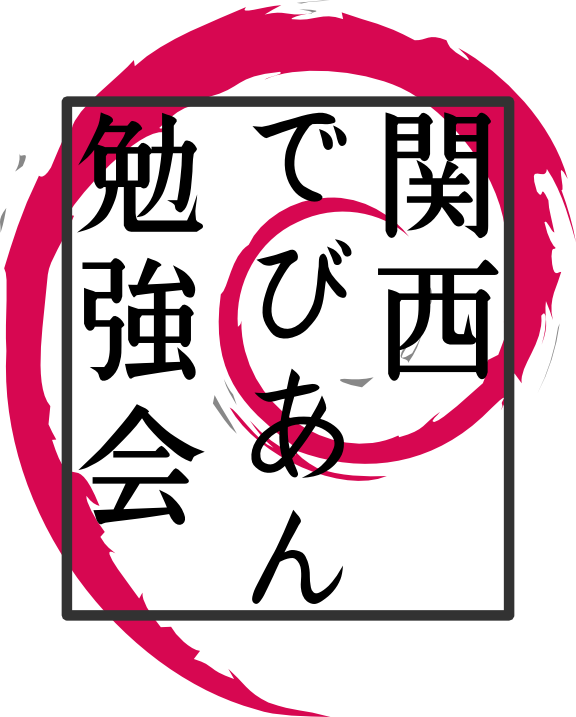
\includegraphics{image200802/kansaidebianlogo.png}
\end{center}

\begin{flushright}
\hfill{}関西 Debian 勉強会担当者 佐々木・倉敷・のがた・かわだ・おおつき \\
\hfill{}\debmtgyear{}年\debmtgmonth{}月\debmtgdate{}日
\end{flushright}

\thispagestyle{empty}
\end{titlepage}

\dancersection{最近のDebian関係のイベント報告}{Debian JP}

\dancersection{事前課題}{関西Debian勉強会}

参加者の皆さんは以下の通りです:
\begin{prework}{Katsuki Kobayashi}
\end{prework}

\dancersection{\mbox{Rustで書いたツールの}\mbox{debianパッケージングに}\mbox{挑戦してみた話(仮)}}{小林 克希}

\subsection{はじめに}

今回の内容ですが、最近個人的に触りだしたRustというプログラミング言語について、
そもそもどういう言語なんだというご紹介(といっても、私も勉強中の身ですが)と、
Rustで書いたツールのdebを作ってみる、というところまでを目標としています。

\subsection{Rustとは}

Rustとは、MozillaがブラウザエンジンServoのために開発したシステムプログラミング言語です。
2018年のスタックオーバーフローの調査%
\footnote{\url{https://insights.stackoverflow.com/survey/2018}}%
で愛されている言語ランキング1位になるなど、
最近では結構メジャーになっていている感じの言語です。
特徴としては、安全性・並行性について考えられて設計されている点で、
かつ、みんな大好き(?)静的型付け言語です。

なお、Rustプログラマーの事をrustacean(ラストシアン)というようです。
これは、``Crustacean(甲殻類)`` から来ているらしく、
そのせいか、オライリー本の表紙はオオヒロバオウギガニというカニですし、
非公式マスコットもかわいらしいカニ(名前はFerris%
\footnote{\url{http://rustacean.net/}}%
)になってます。

\subsubsection{Rustのツールチェーンをインストール}

ではさっそくRustのツールチェーンをインストールしてみましょう。
さて、もちろんRustのツールチェーンのdebianパッケージはありますし、
ローカルマシンにインストールせずにブラウザで色々試せるサイト%
\footnote{\url{https://play.rust-lang.org/}}
もあるのですが、Rustは2018年の年末に2018 Edition%
\footnote{\url{https://blog.rust-lang.org/2018/12/06/Rust-1.31-and-rust-2018.html}}%
という大きめな改版があったので、
ひとまずRust公式の手段でツールチェーンをインストールしましょう。
例によって例のごとく、皆様の大事なホームディレクトリに色々と入れてしまいますが、
バージョンアップの頻度はそれなりにあるので、Rustの最新を追っていくなら、
無理せずに公式のツールチェーンを入れてしまった方が無難かと思います。

Rustのツールチェーンですが、以前はそうでもなかったみたいですが、最近ではrustup%
\footnote{\url{https://rustup.rs/}}%
というインストーラーを使うのが公式手順のようです。
いかにも最近のツールっぽいですが、以下のようにcurlコマンドを叩いてインストールします。

\begin{commandline}
% curl https://sh.rustup.rs -sSf | sh
\end{commandline}

rustupを使うと、バイナリは \verb|~/.cargo| 以下にインストールされます。
パスを通したい場合、 \verb|~/.cargo/env| というファイルがあるので、
そちらを \texttt{source} してあげるとよろしいかと思います。
ひとまず、 \texttt{cargo} というコマンドが使えるようになっていたら大丈夫です。
なお、「どうしてもdebで」という方は \texttt{cargo} パッケージをインストールしてください。
その際、\texttt{rustc}のバージョンが2018 Editionである1.31以降である事が望ましいです。

\subsubsection{Hello Worldしてみる}

では、cargoが使えるようになったところで、Hello Worldしてみましょう。
Rustのプロジェクトは、 \verb|cargo new| で作成することができます。
昔は\verb|--bin|をつけないとライブラリ用のプロジェクトになってましたが、
最近のcargoであればデフォルトがバイナリ用のプロジェクトになります。
それでは実行してみましょう。

\begin{commandline}
% cargo new hello
     Created binary (application) `hello` package
% tree
.
├── Cargo.toml
└── src
    └── main.rs

1 directory, 2 files
\end{commandline}

実行すると、こんな感じにCargo.tomlというファイルと、
main.rsというソースファイルが作成されます。
そう、Rustのソースファイルの拡張子は.rsです。
そのため、Rustのプロジェクトのウェブサイトは、.rsドメインで作られてる事がおおいです。
ちなみに、.rsはセルビアのドメインです。

実は、この時点でHello Worldの半分が完了しています。
src/main.rsの中身を見てみましょう。

\begin{commandline}
fn main() {
    println!("Hello, world!");
}
\end{commandline}

なんと、既にHello Worldのコードが生成されています。
なお、詳細は省きますが、 \verb|println!()| は関数に見えますが、
ビックリマークが付いている物は、Rustではマクロであったりします。
まぁ、深く付き会う前は、特に気にしなくて良いかと思います。
ビルドして実行するには \verb|cargo run| すればOKです。

\begin{commandline}
% cargo run
   Compiling hello v0.1.0 (/path/to/hello)
    Finished dev [unoptimized + debuginfo] target(s) in 0.31s
     Running `target/debug/hello`
Hello, world!
\end{commandline}

\subsection{Rustの構文等の紹介}

それでは、ここからは簡単にRustの構文等の紹介をしていきたいと思います。
なお、私も勉強中の身ですので、微妙に嘘を書いていたらすいません。
正確な事は、The Book%
\footnote{\url{https://doc.rust-lang.org/book/}}%
と呼ばれる気合の入ったドキュメントがありますのでそちらを参考にしていただけたらと思います。

なお、Rustは比較的学習が難しいとか言われてますが、
なんで難しいのかについて、個人的にはオライリーのRust本で引用されてるQuoraに書かれたコメント%
\footnote{\url{https://www.quora.com/What-do-C-C++-systems-programmers-think-of-Rust/answer/Mitchell-Nordine}}%
がしっくり来たので引用しておきます。
\begin{quotation}
I've found that Rust has forced me to learn many of the things that I was slowly learning as
``good practise'' in C/C++ before I could even compile my code.
\end{quotation}
私は最近会社の仕事の関係でC++の勉強もするハメになってるのですが、まさに上記と同じ感想です。
なにか、C++がこなれて来て、C++11あたりでようやく良い感じになった機能だけを取り入れていったのが
Rustなんじゃないかなぁと。

\subsubsection{変数宣言}

変数の宣言は\texttt{let}キーワードを使います。
型は、最近の言語っぽくコロンの後に書きますが、型が推論できるなら省略可能です。
また、シャドーイングすることも可能で、指定がなければimmutableな変数になるので、
mutableな変数を作る場合は\texttt{mut}キーワードを使います。
具体的な例を以下に示します。

\begin{commandline}
fn main() {
    let x = 1;
    println!("x = {}", x);
    let x = 1.25;
    println!("x = {}", x);
    x = 1;   // エラーになる(そもそもimmutableだけど): expected floating-point number, found integer
    x = 1.5; // エラーになる: cannot assign twice to immutable variable

    let mut y: u32 = 1;
    y -= 1;
    y -= 1;
    println!("y = {}", y);
}
\end{commandline}

例の2つ目の\verb|y -= 1;|ですが、デバッグビルドだとオーバーフローを検知して実行時にパニックを起こします。
リリースビルド(\verb|--release|オプション付きで\texttt{cargo}を実行)だと
パニックは発生しませんが、もちろんおかしな値が表示されます。

なお、基本的な型は以下のようなものがあります。

\begin{quote}
\begin{description}
 \item[整数]
	    \textbf{符号無し:} \texttt{u8}, \texttt{u16}, \texttt{u32}, \texttt{u64}, \texttt{usize}\\
	    \textbf{符号付き:} \texttt{i8}, \texttt{i16}, \texttt{i32}, \texttt{i64}, \texttt{isize}
 \item[浮動小数点] \textbf{単精度:} \texttt{f32}、\textbf{倍精度:} \texttt{f64}
 \item[ブール] \texttt{bool}
 \item[文字] \texttt{char}  (Unicodeの1文字)
 \item[文字列] \texttt{String}
	    \begin{itemize}
	     \item ただし、文字列リテラルの \texttt{str} があってとてもややこしい
	    \end{itemize}
 \item[配列] \texttt{[T; N]} (\texttt{T}: 型,  \texttt{N}: 要素数)
 \item[ベクター] \texttt{Vec<T>} (\texttt{T}: 型)
 \item[スライス] \texttt{\&[T]} (\texttt{T}: 型)
\end{description}
\end{quote}

\texttt{String}と\texttt{str}が少々ややこしいですが、
イメージとしてはC++の\texttt{std::string}と\texttt{char}の関係に近いような感じです。
\texttt{String}の方は可変長で、メモリ上のイメージを図にすると図\ref{fig:str-string}のような感じです。
\texttt{\&}がついてる\texttt{str}は、この後述する参照になってます。
ひとまず、以下がちょっとしたサンプルコードです。

\begin{figure}[htbp]
 \begin{center}
  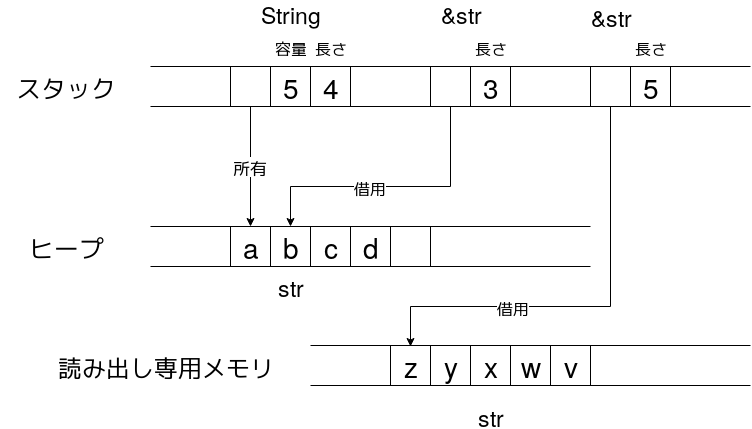
\includegraphics[keepaspectratio,height=4cm]{./image201903/rustlang-str-string.png}
  \label{fig:str-string}
  \caption{RustにおけるStringとstrの違い}
 \end{center}
\end{figure}

\begin{commandline}
fn main() {
    let a = "abcd".to_string(); // String::from("abcd"); でも可
    let b = &a[1..];
    let c = "zyxwv";

    let mut a = "abcd".to_string();
    //  ^^^  aをmutableな変数として宣言
    a.push_str("efg");  // OK

    let mut c = "zyxwv";

    // エラー!: no method named `push_str` found for type `&str` in the current scope
    c.push_str("ut");  // strには追加できないのでpush_strメソッドはない
}
\end{commandline}

\subsubsection{関数定義}

では、関数を定義してみましょう。
Rustでの関数定義は、\texttt{fn}キーワードと`\texttt{->}'トークンを使います。
まずは、単純に足し算を行う関数\texttt{add}を定義してみます。

\begin{commandline}
fn add(a: i32, b: i32) -> i32 {
    return a + b;
}

fn main() {
    println!("{}", add(1, 2));
}
\end{commandline}

これを\texttt{cargo}で実行すると、
(驚くような事は一切ないですが)以下のような結果になります。

\begin{commandline}
% cargo run
Compiling function v0.1.0 (/path/to/examples/function)
Finished dev [unoptimized + debuginfo] target(s) in 0.20s
Running `target/debug/function`
3
\end{commandline}

なお、ここでは\texttt{return}を使いましたが、
Rustではセミコロンを抜かすと値を作るため、
セミコロンを抜かして書いた以下のような\texttt{add}関数も
上記で定義した関数と同じ動作をします(セミコロンを書くとエラーになります)。

\begin{commandline}
fn add(a: i32, b: i32) -> i32 {
    a + b
}
\end{commandline}

\subsubsection{所有権}

さて、ここから一気にRustっぽい話になります。
Rustでは、メモリの安全性が考えられていると書きましたが、
そのために所有権(英語ではownership)という概念を使っています。
C++でもある概念ですが、たとえば以下のようなプログラムがあったとします。

\begin{commandline}
fn main() {
    let i0 = 1;
    let i1 = i0;
    let i2 = i0;

    let s0: String = "hoge".to_string();
    let s1 = s0;
    let s2 = s0;
}
\end{commandline}

さて、どうなると思うでしょうか?
正解は、以下のように\texttt{s2}に\texttt{s0}を代入しているところでエラーになります。

\begin{commandline}
error[E0382]: use of moved value: `s0`
 --> ownership/src/main.rs:8:15
  |
6 |     let s0: String = "hoge".to_string();
  |         -- move occurs because `s0` has type `std::string::String`, which does not implement the `Copy` trait
7 |     let s1 = s0;
  |              -- value moved here
8 |     let s2 = s0;
  |              ^^ value used here after move
\end{commandline}

Rustでは、代入、関数の引数、関数の戻り値などで値の所有権が移動するため、
一度所有権を移譲してしまったら、移譲元の変数はその後アクセスできなくなります(コンパイル時に怒られる)。
ところが、上記のコードでは整数の方はエラーになりません。
これは何故かというと、整数など一部の型(サイズが固定で小さいものが主?)は移動せずにコピーになります。
実はエラーメッセージにあるCopy traitというのがミソで、
整数型はこのCopy traitを実装しているからそういった動作になっています。
traitについては後述します。

関数の引数でも所有権は移動するので、以下のようなコードもアウトです。

\begin{commandline}
fn consume(_s: String) {}

fn main() {
    let h: String = "Hello World".to_string();
    consume(h);
    let hh = h;
}
\end{commandline}

ビルドすると、関数\texttt{consume}コール時に\texttt{h}が移動してしまっているため
以下のようなエラーになります。

\begin{commandline}
12 |     let h: String = "Hello World".to_string();
   |         - move occurs because `h` has type `std::string::String`, which does not implement the `Copy` trait
13 |     consume(h);
   |             - value moved here
14 |     let hh = h;
   |              ^ value used here after move
\end{commandline}

逆に、関数の戻り値でも所有権を移動できるので、以下のようなコードが書けたりします。

\begin{commandline}
fn generate(i: i32) -> Vec<i32> {
    let mut v = Vec::new();
    v.push(i);
    return v;
}

fn main() {
    let v1 = generate(10);
    let mut v2 = generate(100);
    v2.push(101);
    println!("v1: {:?}", v1); // v1: [10]
    println!("v2: {:?}", v2); // v2: [100, 101]
}
\end{commandline}

\subsubsection{参照と借用}

関数呼び出しなどでは、所有権を渡さずに値を使いたい場合が多々あるかと思いますが、
その場合には参照を使います。
なお、Rustでは借用とも言います。
記法としては、C++と同じく\texttt{\&}を使うのですが、
C++とは、
\begin{itemize}
 \item 借用する側(参照される側)に`\texttt{\&}'を付ける
 \item 関数の呼び出し元と呼び出し先両方に`\texttt{\&}'が必要
\end{itemize}
といった点で異なる感じになります。
先程、所有権の移動でエラーになった関数呼び出しのコードを
参照をつかってエラーにならないように書き換えたものが以下になります。

\begin{commandline}
fn consume(_s: &String) {}

fn main() {
    let s0: String = "hoge".to_string();
    let s1 = &s0;
    let s2 = &s0;

    let h: String = "Hello World".to_string();
    consume(&h);
    let hh = h;
}
\end{commandline}

このコードであれば、関数\texttt{consume}をコールしても、
\texttt{h}の所有権はうつっていないため、その後\texttt{hh}に所有権を移譲することができます。
参照の解決には、以下のように\texttt{*}を使います。

\begin{commandline}
fn main() {
    let i0 = 5;
    let i1 = &i0;

    println!("i0: {}, i1: {}", i0, *i1);
}
\end{commandline}

が、関数で使う場合だったり、色々な場面で省略できたりするみたいです。

\begin{commandline}
fn catlength(a: &String, b: &String) -> usize {
    return a.len() + b.len();
}

fn main() {
    let s0 = "hoge".to_string();
    let s1 = "fuga".to_string();
    println!("{}", catlength(&s0, &s1));
}
\end{commandline}

\subsubsection{ライフタイム}

Rustには、GCはなくてC言語のように変数スコープがあり、
スコープを外れた変数は随時消えていきます。
例としては、以下のようなコードを書くと、
ドロップされた後に値を使おうとしているためコンパイル時の怒られます。

\begin{commandline}
fn main() {
    {
        let a = 0;
    }  // ここでドロップ
    println!("{}", a);
}
\end{commandline}

実行すると以下のように怒られます。

\begin{commandline}
error[E0425]: cannot find value `a` in this scope
--> lifetime/src/main.rs:5:20
  |
5 |     println!("{}", a);
  |                    ^ not found in this scope
\end{commandline}

参照している場合とて怒られます。
例として、以下のようなコードを書きます。

\begin{commandline}
fn main() {
    let r;
    {
        let b = 0;
        r = &b;
    }
    println!("{}", r);
}
\end{commandline}

コンパイル時に怒られます。

\begin{commandline}
error[E0597]: `b` does not live long enough
--> lifetime/src/main.rs:11:9
   |
11 |         r = &b;
   |         ^^^^^^ borrowed value does not live long enough
12 |     }
   |     - `b` dropped here while still borrowed
13 |     println!("{}", r);
   |                    - borrow later used here
\end{commandline}

でも、実はこの\textbf{「コンパイル時の怒られる」}というのがミソなのです。
C/C++でよくやる解放済みのメモリアクセスとかが
コンパイル時にみつかるのです。素敵!!
とはいえ、ややこしいのが関数です。以下がエラーになります。

\begin{commandline}
fn longest(x: &str, y: &str) -> &str {
    if x.len() > y.len() {
        x
    } else {
        y
    }
}
\end{commandline}

こんな感じで怒られます。

\begin{commandline}
error[E0106]: missing lifetime specifier
--> lifetime/src/main.rs:1:33
  |
1 | fn longest(x: &str, y: &str) -> &str {
  |                                 ^ expected lifetime parameter
  |
= help: this function's return type contains a borrowed value, but the signature does not say whether it is \
borrowed from `x` or `y`
\end{commandline}

このコードの問題はなにかというと、
実行するまで\texttt{x}と\texttt{y}(どちらも参照)のどちらを返すかわからないので、
戻り値のライフタイムがどうなるかわからないので、
その後の処理がチェックできないという事で怒られています。
ではどうするかというと、コンパイラが言っている通りlifetime parameterを追加します。
具体的には、生存期間\texttt{'a}という表現を用いて以下のように書きます。

\begin{commandline}
fn longest<'a>(x: &'a str, y: &'a str) -> &'a str {
    if x.len() > y.len() {
        x
    } else {
        y
    }
}
\end{commandline}

これによって、この関数\texttt{longest}の戻り値は、
\texttt{x}か\texttt{y}の短い方のライフタイム以上のライフタイムを持つという記載になり、
コンパイラはこれによって値の借用のチェックを行ないます。

\subsubsection{構造体}

Rustにはclassがなく、構造体\texttt{struct}を使います。
定義はC言語の構造体と同じような(型は後置になります)感じですが、
宣言する場合は各要素の名前を逐一書く必要があります。
ただし、要素名と同名の変数で初期化するときのみ省略可能です。
あとは、他の変数から値をコピーして一部だけ値を入れるといった記法もあります。

\begin{commandline}
struct Point {
    x: f64,
    y: f64,
}

fn main() {
    let _p0 = Point { x: 1.0, y: 1.0 };

    let x = 0.0;
    let y = 0.0;
    let _p1 = Point { x, y }; // 変数名とメンバー名が一緒
}
\end{commandline}

なお、構造体ですが、メソッドを生やすことができます。
その際、\texttt{impl}キーワードを用いて、構造体の定義から離れた場所に書きます。
各関数の最初の引数は特別な引数である\texttt{self}への参照である必要があります。
メンバーの値を書き換えたい場合は\texttt{mut}を付けます。

\begin{commandline}
struct Point {
    x: f64,
    y: f64,
}

impl Point {
    fn abs(&self) -> f64 {
        (self.x * self.x + self.y * self.y).sqrt()
    }
}

fn main() {
    let p0 = Point { x: 1.0, y: 1.0 };
    println!("{}", p0.abs()); // => 1.4142135623730951
}
\end{commandline}

\subsubsection{ジェネリック}

C++のテンプレートやJavaのジェネリクスのように、
Rustでも型だけ異なるような関数や構造体を一般的な形で記述することができます。

\begin{commandline}
struct GenPoint<T> {
    x: T,
    y: T,
}

fn main() {
    let _p1 = GenPoint::<i32> { x: 1, y: 1 };
    let _p2 = GenPoint { x: 1, y: 1 };
    let _p3 = GenPoint { x: 1.5, y: 2.0 };
}
\end{commandline}

\subsubsection{trait}

JavaやGoのインターフェース的なものとして、Rustにはトレイト(trait)というものがあります。
さきほど出てきたCopy traitもこれになります。
トレイトは\texttt{trait}キーワードで定義しますが、
たとえばダックタイピングなtraitを書くと以下のようになります。

\begin{commandline}
// Duckは……
trait Duck {
    fn walk(&self);   // walkして
    fn quack(&self);  // quackするもの!!
}
\end{commandline}

この状態で、このDuck traitを実装する構造体を\texttt{impl}キーワードで以下のように作成します。

\begin{commandline}
struct RealDuck {}

impl Duck for RealDuck {
    fn walk(&self) {
        println!("duck walking");
    }

    fn quack(&self) {
        println!("quack")
    }
}

struct Dog {}

impl Duck for Dog {
    fn walk(&self) {
        println!("dog walking");
    }

    fn quack(&self) {
        println!("bow")
    }
}
\end{commandline}

そうすると、以下のように\texttt{Duck}型を引数とする関数\verb|test_duck()|に
\texttt{RealDuck}と\texttt{Dog}のどちらも渡すことができるようになります。

\begin{commandline}
fn test_duck(duck: &Duck) {
    duck.walk();
    duck.quack();
}

fn main() {
    let duck = RealDuck {};
    let dog = Dog {};

    test_duck(&duck);
    test_duck(&dog);
}
\end{commandline}

なお、引数に複数のtraitを実装した型を要求することができます。
たとえば、
\begin{commandline}
fn notify(item: impl Summary + Display) {
\end{commandline}
は2つのtrait、\verb|Summary|と\verb|Display|を同時に実装した型を引数\texttt{item}に要求します。
これだと読みづらい感じもするので、以下の書き型もできます。
\begin{commandline}
fn notify<T: Summary + Display>(item: T) {
\end{commandline}
また、引数が一杯になってきたら上記でも辛いので、以下のような\texttt{where}をつかって記法もあります。
\begin{commandline}
fn some_function<T, U>(t: T, u: U) -> i32
    where T: Display + Clone,
          U: Clone + Debug
{
\end{commandline}

\subsubsection{enum}

さて、enumです。個人的にはかなり気にいってますが、
Rustのenumは、ちょっとおかしなくらいに色々とできます。
もちろん、C言語のような以下のようなenumは作れます。

\begin{commandline}
enum Fruits {
    Apple,
    Banana,
    Orange,
    Peach,
}

fn main() {
    let _hoge = Fruits::Apple;
}
\end{commandline}

が、Rustのenumは、各値の中にさらに値を持たせることができます。
しかも、型や値の個数はバラバラで構いません。
たとえば、以下のようなenumを定義できます。
なお、ここで出てきている\texttt{(u8, u8, u8, u8)}というのは
8-bit符号無し整数を4つ持つタプル型です。

\begin{commandline}
enum IpAddr {
    V4((u8, u8, u8, u8)),
    V6(String),
}
\end{commandline}

このように定義してあげると、実際の値を作る際、
以下のように値を入れてenumの値を作ることができます。

\begin{commandline}
fn main() {
    let v4_addr = IpAddr::V4((127, 0, 0, 1));
    let v6_addr = IpAddr::V6("::1".into());
}
\end{commandline}

このようにして作った値は、\texttt{match}を使って値を取り出せます。
C言語の\texttt{switch}文的な感じで使えます。
以下のコードはenum値全てのケースを記述していますが、
\texttt{default}的な処理は``\verb|_ => { /* 処理 */ }|''として書けます。

\begin{commandline}
fn extract_addr(addr: &IpAddr) {
    match addr {
        IpAddr::V4(a) => {
            println!("{}.{}.{}.{}", a.0, a.1, a.2, a.3);
        }
        IpAddr::V6(a) => {
            println!("{}", a);
        }
    }
}

fn main() {
    extract_addr(&v4_addr); // => 127.0.0.1
    extract_addr(&v6_addr); // => ::1
}
\end{commandline}

\subsubsection{\texttt{Option<T>}と\texttt{Result<T,E>}}

Rustには例外もnullptrもありませんが、その代わりにジェネリックなenumである
\texttt{Option<T>}と\texttt{Result<T,E>}を使ってエラー等を処理します。
それぞれの機能をざっくり説明すると、
\begin{itemize}
  \item \verb|Option<T>|
	\begin{itemize}
	 \item 値がない可能性がある事を示す (nullptrの代わり)
	\end{itemize}
 \item \verb|Result<T,E>|
       \begin{itemize}
	\item 失敗する可能性がある事を示す (例外の代わり)
       \end{itemize}
\end{itemize}
といった感じでしょうか。
それぞれの定義は以下のようにされています。

\begin{commandline}
pub enum Option<T> {
    None,
    Some(T),
}

pub enum Result<T, E> {
    Ok(T),
    Err(E),
}
\end{commandline}

例えば、1つ目のコマンドライン引数を受けとり、
それをi32型に変更して表示する関数を書くと次のようになります。
まず引数が一つも無い場合があるため、引数があれば\texttt{Some()}の中身に引数が、
なければ\texttt{None}が取り出されます。
その後、\texttt{Some()}の中身を取り出しますが、
i32型としてパースできない場合があるため、成功したか失敗したかを
\texttt{Ok()}か\texttt{Err()}かで判定しています。

\begin{commandline}
use std::env;

fn main() {
    let i = match env::args().nth(1) {
        None => {
            panic!("no arguments");
        }
        Some(arg) => match arg.parse::<i32>() {
            Ok(fig) => fig,
            Err(e) => {
                panic!("error: {}", e);
            }
        },
    };

    println!("i: {}", i);
}
\end{commandline}

実際には、上記の処理をもうちょっと綺麗に書けるように
\texttt{?}演算子や\texttt{expect()}メソッドなどが定義されています。
が、ここでは詳細は省きます。

\subsubsection{crate}

Rustのプログラムは、クレート(crate)と呼ばれる単位の組み合わせで構成されます。
今回は、詳細については割愛して、
crates.io\footnote{\url{https://crates.io/}}にて公開されている
クレートの使い方について簡単に紹介します。
といっても、実はとても簡単で、cargoの設定ファイルのCargo.tomlに
crates.ioで使いたいクレートのページに掲載されている式を貼り付けるだけです。

今回はオプション解析のクレートであるclap\footnote{\url{https://clap.rs/}}を使ってみましょう。
サイトにある式を、Cargo.tomlの[dependencies]の項目に追記してあげればOKです。

\begin{commandline}
[dependencies]
clap = "2.32.0"
\end{commandline}

では、これをつかって、簡単なプログラムを作ってみます。
とりあえず、\verb|-n|オプションだけあるような
似非echoコマンドを以下のように書いてみました。

\begin{commandline}
use clap::{App, Arg};

fn main() {
    let m = App::new("echo")  // コマンド名
        .arg(Arg::with_name("STRING").multiple(true))  // 複数の引数
        .arg( // '-n' を定義
            Arg::with_name("n")
                .short("n")
                .help("do not output the trailing newline"),
        )
        .get_matches();  // 実行

    let out = match m.values_of("STRING") {
        //         ↓地味にイテレータを使用
        Some(v) => v.collect::<Vec<&str>>().join(" "),
        None => "".into(),
    };

    print!("{}", out);

    if !m.is_present("n") {
        println!("");  // '-n'オプションがなければ改行
    }
}
\end{commandline}

Rust 2018 Editionと呼ばれる2018年の年末にリリースされたバージョン以降では、
これまで必要だった\verb|extern crate clap;|という記述が不要になっています。

ということで、ここまでかなり高速にRustの構文等の紹介をしてきましたが、
まったくもって極一部ですので、興味があればThe Bookを読んでもらえればと思います。

\subsection{Debianパッケージにしてみる}

ここでようやくDebianな話題ですが、ひとまずここでは先程作成したclapで作った似非echoコマンドを
debianパッケージにしてみるということをやります。

Rustの単一バイナリのdebianパッケージ化について、
一番簡単なのは\texttt{cargo}のサブコマンド用の
\texttt{cargo-deb}%
\footnote{\url{https://github.com/mmstick/cargo-deb}}%
を用いる方法があるようです。
あるようなんですが……残念ながらこのツール、
とても公式に入れられないようなdebしか吐かないようです。
ドキュメントもないし云々。
まぁ、/usr/binにえいやと入れたいならアリかもですが。

で、さすがにそれだとアレなので、もうちょっとちゃんとしたdebを作るべく、
Debian Rust packaging teamのWiki%
\footnote{\url{https://wiki.debian.org/Teams/RustPackaging}}%
に、それなりにしたがってみようかと思います。
どうやら、crates.ioにあるcrateについては、
debcargo\footnote{\url{https://salsa.debian.org/rust-team/debcargo}}%
というツールを使うと良い感じに処理してくれるようです。
が、今回はcrate.ioにはアップされていないもので作りたいという話なんですが、
debcargoは対応していなさそうです。
そのため、debcargoが使っているdh-cargoをつかって地道に対応してみることにしました。

まずは、dh\_makeを実行してdebianディレクトリを作り、
できあがったdebian/rulesのbuildルールのdhにオプション\verb|--byildsystem cargo|を追加することと、
debian/controlのBuild-Dependsにdh-cargoとlibrust-clap-devを追加してみました。
ひとまずここでビルドしてみます。

\begin{commandline}
% debuild-pbuilder
-> Attempting to satisfy build-dependencies
-> Creating pbuilder-satisfydepends-dummy package
Package: pbuilder-satisfydepends-dummy
Version: 0.invalid.0

... (snip) ...

dh_autoreconf -O--buildsystem=cargo
dh_auto_configure -O--buildsystem=cargo
cp: './debian/cargo-checksum.json' を stat できません: そのようなファイルやディレクトリはありません
\end{commandline}

なにかファイルがないと言われてしまいました。
Wikiを見ると、どうやらupstreamのcrateのチェックサムを含めたファイルを
用意してやる必要があるようです。
これは、/usr/share/cargo/registry以下にdebでインストールされた
ライブラリたちを使うためのようなのですが、
あまりWikiを読んでも作り方がわかりませんでした。
どうも、cargo-vendorというツールを利用していそうなのですが……。
とか思っていたのですが、

\begin{commandline}
% apt source ripgrep
% cat rust-ripgrep-0.10.0/debian/cargo-checksum.json
{"package":"Could not get crate checksum","files":{}}
\end{commandline}

と、公式のripgrepのdebのソースをみると、このファイルが哀しいことになっていました。
それでもちゃんとビルドは通るようです。
ためしに、debian/cargo-checksum.jsonをtouchで空ファイルとして作ってみたら、
普通にビルドが進んでしまいました。いったんわすれます……。

ところが、まだコケます。

\begin{commandline}
debian cargo wrapper: running subprocess (['env', 'RUST_BACKTRACE=1', '/usr/bin/cargo', '-Zavoid-dev-deps', \
'build', '--verbose', '--verbose', '-j4', '--target', 'x86_64-unknown-linux-gnu'],) {}
error: failed to select a version for the requirement `textwrap = "= 0.10.0"`
candidate versions found which didn't match: 0.11.0
location searched: directory source `/path/to/clap-test/debian/cargo_registry` (which is replacing registry \
`https://github.com/rust-lang/crates.io-index`)
required by package `clap v2.32.0`
\end{commandline}

clapが依存しているtextwrapのバージョンが0.10.0だけど、手元にあるのは0.11.0だと。
たしかに、textwrapのdebのバージョンは0.11.0でした。
が、そうなるとおなじくclapを使っているripgrepのビルドが通っているのが解せません。
と調べていくと、GitHubのリポジトリ\footnote{\url{https://github.com/BurntSushi/ripgrep}}に
置いてあるバージョンとripgrepのdebのorigソースを見比べると、
Cargo.tomlが若干異なり、Cargo.lockが編集されていることがわかりました。
そして、消されたCargo.lockの中には、textwrapの0.10.0のチェックサムが記載されています。
そもそも、Cargo.tomlはで開発者がざっくりとした依存を書くファイルで、
Cargo.lockは、cargoが実情に基づいて自動で生成し、
\verb|cargo update|などすることによってバージョンが更新されるものです。

で、確認していくと、どうやら/usr/share/cargo/registry以下にあるtextwrapの
Cargo.tomlのtextwrapの依存がcrates.io登録時に以下のように書きかわっていることがわかりました。

\begin{commandline}
% grep -A 1 dependencies.textwrap debian/cargo_registry/clap-2.32.0/Cargo.toml
[dependencies.textwrap]
version = ">= 0.10, < 0.12"
\end{commandline}

ちなみに、GitHubのclapのコードには以下としか書いてないです。

\begin{commandline}
[dependencies]
bitflags              = "1.0"
unicode-width         = "0.1.4"
textwrap              = "0.10.0"
\end{commandline}

ということで、変更の基準はまったくわかってませんが(今後の課題とさせていただきます!!)、
今回の似非echoコマンドについては、Cargo.lockを消せば最後までビルドされました。
lintianのエラーも警告も取れてないですが、ひとまず動きますよ!!

\begin{commandline}
% dpkg -I rust-clap-test_0.1.0-1_amd64.deb
new Debian package, version 2.0.
size 258160 bytes: control archive=648 bytes.
360 バイト、   11 行      control
285 バイト、    4 行      md5sums
Package: rust-clap-test
Version: 0.1.0-1
Architecture: amd64
Maintainer: Katsuki Kobayashi <rare@tirasweel.org>
Installed-Size: 770
Depends: libc6 (>= 2.18), libgcc1 (>= 1:4.2)
Section: unknown
Priority: optional
Homepage: <insert the upstream URL, if relevant>
Description: <insert up to 60 chars description>
<insert long description, indented with spaces>

% dpkg -c rust-clap-test_0.1.0-1_amd64.deb
drwxr-xr-x root/root         0 2019-03-23 18:06 ./
drwxr-xr-x root/root         0 2019-03-23 18:06 ./usr/
drwxr-xr-x root/root         0 2019-03-23 18:06 ./usr/bin/
-rwxr-xr-x root/root    776600 2019-03-23 18:06 ./usr/bin/clap-test
drwxr-xr-x root/root         0 2019-03-23 18:06 ./usr/share/
drwxr-xr-x root/root         0 2019-03-23 18:06 ./usr/share/doc/
drwxr-xr-x root/root         0 2019-03-23 18:06 ./usr/share/doc/rust-clap-test/
-rw-r--r-- root/root       197 2019-03-23 18:06 ./usr/share/doc/rust-clap-test/README.Debian
-rw-r--r-- root/root       190 2019-03-23 18:06 ./usr/share/doc/rust-clap-test/changelog.Debian.gz
-rw-r--r-- root/root      1693 2019-03-23 18:06 ./usr/share/doc/rust-clap-test/copyright
\end{commandline}

\subsection{まとめ}

ということで、しりすぼみ感は拭えませんが、
結局Rustなdebを作るには、現状ではcrates.ioに登録してdebcargoをベースにつくる
というのが公式のようでした。
が、もちろんdh-cargoがあるのでcrates.ioに登録しなくてもdebにはできそうです。
cargo自体は、外部クレートにgitリポジトリを指定したりできるので、
debcargoもgitリポジトリに対応できたら良いですが、今回のCargo.toml/Cargo.lockを
crates.ioが編集している兼ね合いもあるので、色々と大変かもしれません。

というか、そもそもlibrust-*パッケージ達の依存関係はあやしいのかもしれません。
つい先日も、ripgrepがビルドできないというバグも報告されていましたし%
\footnote{\url{https://bugs.debian.org/cgi-bin/bugreport.cgi?bug=920958}}。
とは言え、debcargo自体は粛々と開発が進んでいるようで、
これを書いてる直前くらいにも、busterには入らないけど
post-installでtestができるようになったり%
\footnote{\url{https://alioth-lists.debian.net/pipermail/pkg-rust-maintainers/2019-March/005296.html}}%
しているようです。
なんにせよ、Rust自体は良い言語かと思うので、
今後流行っていけば良いなぁと思います。

\clearpage

\dancersection{開催の予定}{}


\vspace{\fill}
本資料は GPL v 2.0 のライセンスで公開いたします。

\clearpage

%
% 冊子にするために、4の倍数にする必要がある。
% そのための調整

\mbox{}\newpage
\mbox{}\newpage

\printindex
%\cleartooddpage

 \begin{minipage}[b]{0.2\hsize}
  \rotatebox{90}{\fontsize{80}{80} {\gt 関西 Debian 勉強会} }
 \end{minipage}
 \begin{minipage}[b]{0.8\hsize}

 \vspace*{15cm}
 \rule{\hsize}{1mm}
 \vspace{2mm}
 
\includegraphics[width=2cm]{image200502/openlogo-nd.eps}
 \noindent \Large \bfseries{Debian 勉強会資料}\\ \\
 \noindent \normalfont \debmtgyear{}年\debmtgmonth{}月\debmtgdate{}日 \hspace{5mm}  初版第1刷発行\\
 \noindent \normalfont 関西 Debian 勉強会 (編集・印刷・発行)\\
 \rule{\hsize}{1mm}
 \end{minipage}

\end{document}




